\documentclass{uflamon}          % classe base para a monografia

%==============================================================================
% Utilizacao de pacotes
\usepackage[T1]{fontenc}         % usa fontes postscript com acentos
\usepackage[brazil]{babel}       % hifenização e títulos em português do Brasil
\usepackage[utf8]{inputenc}     % permite edição direta com acentos
\usepackage{amsmath}             % pacote da AMS para Matemática Avançada
\usepackage{amssymb}             % símbolos extras da AMS
\usepackage{latexsym}            % símbolos extras do LaTeX
\usepackage{graphicx}            % para inserção de gráficos
\usepackage{listings}            % para inserção de código
\usepackage{fancyvrb}            % para inserção de saídas de comandos
%\usepackage{enumerate}           % para personalizar lista enumeradas 
											%(incluso na classe)
\usepackage{longtable}           % para tambelas muito grandes NOVO!!!!

\usepackage{colortbl} % cores em tabelas
\newcolumntype{Z}{|>{\columncolor[gray]{0.9}}l|} %cor cinza em células
%\usepackage{array} % já incluso na classe
\newcolumntype{L}[1]{>{\raggedright\let\newline\\\arraybackslash\hspace{0pt}}m{#1}}
\newcolumntype{C}[1]{>{\centering\let\newline\\\arraybackslash\hspace{0pt}}m{#1}}
\newcolumntype{R}[1]{>{\raggedleft\let\newline\\\arraybackslash\hspace{0pt}}m{#1}}
\usepackage{multirow} % para juntar duas linhas em uma só
\usepackage{multicol} % para uso de várias colunas

% cores para os links cruzados
\usepackage{color}
\definecolor{rltred}{rgb}{0.2,0,0}
\definecolor{rltgreen}{rgb}{0,0.2,0}
\definecolor{rltblue}{rgb}{0,0,0.2}

\usepackage[colorlinks=true,
            urlcolor=rltblue,       % \href{...}{...} external (URL)
            filecolor=rltgreen,     % \href{...} local file
            linkcolor=rltred,       % \ref{...} and \pageref{...}
            citecolor=rltgreen,
            pdftitle={Pr\'e-Projeto --AAS. Projetos em Qu\'imica Experimetal},
          pdfauthor={Marcus Bruno Fernandes Silva},
          pdfsubject={projeto sobre AAS},
          pdfkeywords={aas}%
]{hyperref} % para referência cruzadas
%\usepackage{hyperref}            % para referência cruzadas
\usepackage{subfigure}           % figuras dentro de figuras
\usepackage{caption}            % remodelando o formato dos títulos de 
                                 % tabelas e figuras

% configuração padrão do listings   
\lstset{
   language=Java,
   extendedchars=true,
   tabsize=3,
   basicstyle=\footnotesize\ttfamily,
   stringstyle=\em,
   showstringspaces=false 
}

% para referências de acordo com a ABNT
% precisa instalar o abntex2 antes!!!
% http://abntex.codigolivre.org.br/
% comente se pretende usar outro padrão

%abnt-emphasize=bf coloca o título das bibliografias em negrito
%abnt-thesis-year=both
\usepackage[alf,num,abnt-etal-cite=3,abnt-etal-list=3,abnt-url-package=url,abnt-emphasize=bf]{abntex2cite}

% evite usar o hyperref com abntex, pode dar caca em urls... no linha anterior, informo
% para incluir urls usando o pacote url e não o hyperref
%
% caso queira o hyperref com abntex, comente a linha anterior e descomente a seguinte
%\usepackage[alf,abnt-etal-cite=3,abnt-etal-list=0,abnt-etal-text=emph]{abntex2cite}
%
% caso vc ainda use a versão anterior da abntex, comente a linha incluindo o abntex2cite
% e descomente a próxima linha 
%\usepackage[alf,abnt-etal-cite=3,abnt-etal-list=0,abnt-etal-text=emph]{abntcite}


% redefinindo formatação de títulos de tabelas e figuras

%==============================================================================
\usepackage{microtype} 			% para melhorias de justificação
\usepackage{float}
\usepackage{titling}

% Especificando hifenizações que por ventura LaTeX não saiba fazer
% Por padrão 99,9% dos termos em português devem ser hifenizados corretamente.
\hyphenation{hardware software Li-nux am-bien-te diag-nos-ti-car coor-de-na-ção 
FAE-PE Recovery TelEduc Williams UFLA Sérgio}

%==============================================================================
% Dados da monografia, capa: autor, titulo, banca, etc... - SUBSTITUA DE ACORDO
%==============================================================================
\author{Gabriela Nunes \\
       Gustavo Henrique de Souza Paiva \\
       Larissa Souza Castro \\
       Marcus Bruno Fernandes Silva}
\subtitle{Exemplo para os Usuários}
%\author{Joao}
\title{Determinação de Ácido Acetilsalicílico em Medicamentos}
\engtitle{Use of Uflamon Class}
%\engsubtitle{Sample for Users}
%\edicao{3$^a$ edição revista, atualizada e ampliada}
\date{2017}
\tipo{Pré-projeto entregue e apresentado ao Professor Sérgio, como requisito da disciplina.}
\orientador{Prof. Sergio Scherrer Thomasi}
\newcommand{\orient}{Prof. Sergio Scherrer Thomasi}
\newcommand{\otipo}{Pré-projeto entregue e apresentado ao Professor Sérgio, como requisito da disciplina GQI 169.}
\newcommand{\olocal}{Lavras -- MG}
\local{Lavras -- MG}

%##################################################

\newcommand \fazercapa{
\begin{titlepage}
    \centering

    
\includegraphics[scale=0.45]{logoufla}%

    \vspace{1cm}

    \Large\theauthor
    
    \vspace{\stretch{1}}

    \bfseries\LARGE\MakeUppercase\thetitle

    \vspace{\stretch{1}}

    \Large\MakeUppercase\olocal\\
    \MakeUppercase\thedate
    \null
    \cleardoublepage
\end{titlepage}
}

\newcommand \fazerfolhaderosto{
    \begin{titlepage}
        \newpage

        \begin{center}
            \MakeUppercase\theauthor

            \vspace{\stretch{1}}

            \textbf{\MakeUppercase\thetitle}

            \vspace{\stretch{1}}
            
            \hfill\begin{minipage}{8cm}{\otipo}\end{minipage} % tipo da monografia

            \vspace{\stretch{.58}}

            \ifthenelse{\equal{\@orientador}{\@empty}} % % se orientador nao existir,
            {}%                                            % nao produza nada
            {\orient\\
             Orientador
            }

            \vspace{\stretch{.86}} 

            \textbf{\MakeUppercase\olocal}\\ 
            \textbf{\MakeUppercase\thedate}
            \end{center}
    \end{titlepage}
}

%==============================================================================
% Começar o documento

\begin{document}

\fazercapa

\fazerfolhaderosto

\tableofcontents

\clearpage

\pagestyle{ufla}

%==============================================================================
% incluindo os capitulos

\chapter{Introdução}\label{intro}
\section{Justificativa}\label{sub:just}    

O ácido acetilsalicílico é, possivelmente, o medicamento mais conhecido e vendido no mundo todo.
Desse modo, a análise dos comprimidos comercializados é de interesse dos estudantes da Engenharia
Química, uma vez que proporciona aprendizado a cerca da indústria farmacêutica, padrões de
qualidade, além de práticas laboratoriais da teoria de química analítica e orgânica.

\section{Objetivos}\label{sub:Objetivos}
Determinar o teor de ácido acetilsalicílico contido nos comprimidos comercializados, analisando
medicamentos de referência (Aspirina\R), genéricos e similares.

\section{Referencial Teórico}\label{sub:reft}

\subsection{Histórico}\label{sub:Histórico}

O ácido acetilsalicílico (AAS) é um dos medicamentos mais populares no mundo, sendo conhecido por
seu nome comercial: Aspirina\R. Ele é um analgésico, anti-inflamatório e antipirético produto de uma
reação que tem como um dos reagentes o ácido salicílico, extraído do salgueiro (\textit{Salix
alba}).  

O ácido acetilsalicílico pode ser identificado também pela sua fórmula química \ce{C9H8O4} e seu
nome IUPAC ácido 2-acetóxibenzóico. É um ácido de caráter fraco por apresentar-se,
predominantemente, em sua forma não ionizada. Demonstra características de um ácido orgânico e de
éster, pois ambas as estruturas existem em sua fórmula molecular. A respeito de propriedades
físico-químicas, o AAS é um pó cristalino branco, inodoro, solúvel em álcool e éter e pouco solúvel
em água devido à massa molar elevada de 180,157g/mol, sendo a relação de sua solubilidade em água
0,3g/100g (25$^\circ$C). Ele possui ponto de fusão 135$^\circ$C e ponto de ebulição a 140$^\circ$C.
Ecologicamente, é facilmente biodegradado em estações de tratamento de água e não
bioacumula.~\cite{teves}

\begin{figure}[H]
\begin{center}
    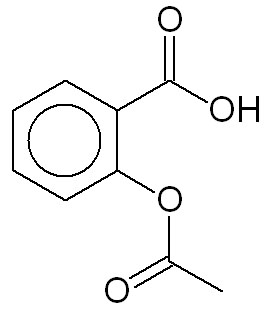
\includegraphics[scale=.4]{figuras/acido_acetilsalicilico.jpg}
\end{center}
\caption{Ácido acetisalicílico}
\label{fig:acid_AAS}
\end{figure}


A utilização do ácido salicílico, no alívio de dores já existe há séculos, isso porque essa
substância está contida em diversas plantas consideradas medicinais. “Uma coleção de anotações
datadas de cerca de 1500 a.C., conhecidas como papiros de Ebers, já recomendava o uso da infusão de
folhas de murta para o alívio de dores reumáticas”~\cite{aspirinabayer}. Posteriormente, no século V
a.C., Hipócrates, o pai da medicina moderna, registrou que o pó da casca do salgueiro era capaz de
amenizar dores e febre. Somente em 1860 a substância encontrada na casca do salgueiro foi isolada em
laboratório e recebeu o nome de salicilato, que designa um “grupo de fármacos que atuam devido ao
seu conteúdo de ácido salicílico”.~\cite{Goodman2005}

Já o descobrimento do ácido acetilsalicílico ocorreu mais tarde, “quando o químico alemão Felix
Hoffman pesquisava um medicamento para ser usado no tratamento da artrite, doença de seu pai. O
objetivo dele era encontrar uma droga para substituir o salicilato de sódio, medicamento usado
naquela época, mas que exigia grandes doses diárias e provocava irritação e fortes dores estomacais
nos pacientes”.~\cite{massabni2006}

Em 1897, Hoffman, que trabalhava na companhia Bayer da Alemanha, preparou o ácido acetilsalicílico
combinando o ácido salicílico com acetato. A reação resultou numa substância mais vantajosa do que o
salicilato de sódio, em questão de eficiência e efeitos colaterais. Tal droga recebeu,
posteriormente, o nome de Aspirina\R e se tornou o primeiro fármaco sintetizado em laboratório.  

A Aspirina\R teve sua patente concedida em 1899 e começou a ser comercializada.  Ainda que
inicialmente os superiores de Hoffman achassem que o medicamento fracassaria, o mesmo tornou-se
sucesso de vendas e inclusive destacou-se como medicamento mais utilizado no tratamento da artrite.
Inicialmente, a Aspirina\R era vendida na forma de pó, entretanto, em 1900, ela tornou-se o primeiro
medicamento no mundo a ser vendido em doses padronizadas, que eram comprimidos com 500mg de ácido
acetilsalicílico. “A formulação em comprimidos tinha três vantagens principais: assegurar que cada
comprimido tivesse uma dose exata do ingrediente ativo, acabar com as falsificações dos produtos e
reduzir os custos de produção".~\cite{aspirinabayer}

Décadas depois, John Vane, Professor de Farmacologia do London Royal College for Surgeons, “observou
que alguns tipos de ferimento eram acompanhados da liberação em nosso corpo de substâncias chamadas
de prostaglandinas. Ele também percebeu que dois grupos delas provocavam febre e vermelhidão no
local do ferimento (sinais de inflamação). Vane e colaboradores descobriram que a Aspirina\R
bloqueava a síntese de prostaglandinas, evitando a formação de plaquetas, que depois se
transformavam em coágulos de sangue no corpo humano. Esses coágulos eram responsáveis pelo bloqueio
do fluxo de sangue para o coração, resultando no ataque cardíaco. Assim, a Aspirina\R evita a
formação de coágulos e, portanto, pode impedir o infarto do miocárdio”~\cite{massabni2006}. Em 1971,
Vane publicou no jornal “Nature” seus estudos sobre o mecanismo de ação do ácido acetilsalicílico,
as descobertas feitas por ele lhe renderam o Prêmio Nobel de Medicina de 1982. 

Nos últimos 30 anos, pesquisa foram feitas com diferentes grupos de pessoas que apresentavam
problemas cardiovasculares, cerebrovasculares e também pessoas sadias. Os resultados mostraram que a
Aspirina\R teve um grande impacto no tratamento e prevenção das doenças cardiovasculares.  Além
disso, pelo fato de ser anticoagulante, há trabalhos que mostram que a Aspirina\R reduz o risco de
trombose e derrame cerebral. No entanto, algumas pessoas podem apresentar efeitos colaterais como
dores estomacais, diarréias, náuseas, sangramento e hemorragia interna. Não é recomendado a sua
utilização para quem possui problemas renais ou gástricos.

\subsection{Síntese de ácido acetilsalicílico}

A síntese da Aspirina\R é dada através de uma reação de acetilação do ácido salicílico, que é um
composto aromático bifuncional, possuindo os grupos fenol e ácido carboxílico. O ácido salicílico é
um ácido orgânico, de fórmula química \ce{C7H6O3}. Ele é sólido em seu estado puro, apresenta-se em
temperatura ambiente na forma de cristais brancos ou de pó cristalino, é pouco solúvel em água, mas
solúvel em solventes polares e éter, devido a polaridade, as forças de atração intermolecular e o
tamanho da cadeia carbônica.

\begin{figure}[H]
\begin{center}
    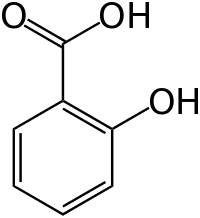
\includegraphics[width=.3\textwidth]{figuras/acido_salicilico.png}
\end{center}
\caption{Ácido salicílico}\label{fig:acid_salicilico}
\end{figure}

A acetilação ou etanoilação é o processo de introdução do grupo acetila (ou etanoila) em um composto
orgânico. O radical acetila possui o grupo metila (\ce{CH3}$-$) conectado por uma ligação simples a um
carbonila. O carbono do grupo carbonila possui um único elétron livre, com o qual forma uma ligação
com o radical R da molécula.

\begin{figure}[H]
\begin{center}
    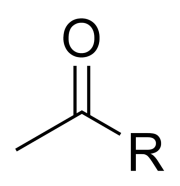
\includegraphics[width=.3\textwidth]{figuras/im1.png}
\end{center}
\caption{Grupo acetila ligado a uma cadeia carbônica.}\label{fig:im1}
\end{figure}

A seguir é explicada uma reação do ácido salicílico com utilização do anidrido acético como agente de
acetilação na produção de ácido acetilsalicílico. Essa síntese é a uma das mais reproduzidas, pois
possui características comerciais que são mais favoráveis às indústrias químicas devido a sua
eficiência e o seu baixo custo. Há a necessidade de um catalisador nessa reação e o descrito no
mecanismo a seguir é o ácido sulfúrico. Resumidamente, a reação entre um anidrido e um álcool (ou
hidroxiácido) gera um ácido carboxílico e um éster. Os ésteres são também derivados de ácido
carboxílico. Eles são majoritariamente apolares e insolúveis em água, entretanto são solúveis em
álcool. Eles se dispõem de pontos de fusão e de ebulição baixos por não apresentarem ligações de
hidrogênio. Sua produção advém da reação de um ácido carboxílico com um álcool, resultando em perda
de água.~\cite{SantosES}

\begin{figure}[H]
\begin{center}
    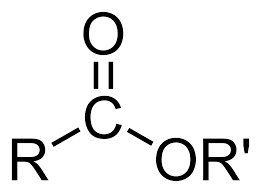
\includegraphics[width=.3\textwidth]{figuras/ester.png}
\end{center}
\caption{Forma generalizada de um éster}
\label{fig:ester}
\end{figure}

Dando início à síntese, o ácido sulfúrico irá agir na reação como um catalisador, sendo assim ele
irá se ionizar liberando um \ce{H+} que se ligará em um dos oxigênios presentes na molécula de
anidrido acético. Quando isso ocorre, o oxigênio que recebeu o hidrogênio deixa de fazer ligação
dupla com o carbono e consequentemente o carbono fica com três ligações, tornando-se um carbocátion.
Como o carbono está instável, ele busca a sua estabilidade na molécula de ácido salicílico com a
qual ele está reagindo. Portanto, o carbono liga-se na hidroxila do ácido salicílico, mas é
importante ressaltar que a hidroxila que ele irá se ligar é a hidroxila ligada diretamente ao anel
benzênico, devido as forças de atração. Na química orgânica, as ligações de acetilação tem
preferências para se ligarem em hidroxilas em posições orto e para, como é o caso do ácido
salicílico (posição orto da hidroxila). A formação da nova molécula de ácido salicílico com o
carbocátion do anidrido acético possui um oxigênio que contém três ligações, o qual se rearranja na
molécula se desprotonando para estabilizar, ou seja, o hidrogênio ligado a ele irá se ligar no
oxigênio que faz parte do anidrido acético, formando assim um ácido acético que irá se desprender da
molécula. A ligação de elétrons que estava ligada com a parte do ácido acético se direciona para o
respectivo carbono que estava fazendo tal ligação, mas antes disso o hidrogênio da hidroxila que
estava ligada a esse carbono volta para o catalisador (formando novamente o \ce{H2SO4}). Como o
carbono recebeu os pares de elétrons e o oxigênio da hidroxila perdeu o seu hidrogênio, acontece uma
dupla ligação entre o carbono e o oxigênio, dando origem a molécula de ácido acetilsalicílico.


% Remover '\newpage' caso a imagem a baixo altera sua posição
\newpage

\begin{figure}[H]
\begin{center}
    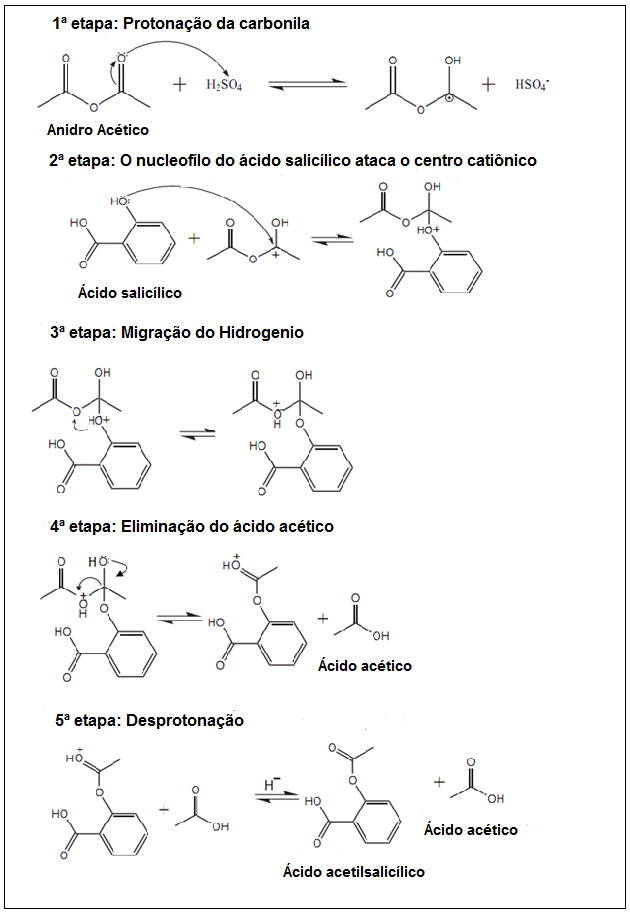
\includegraphics[width=1.1\textwidth]{figuras/im2_sintese.png}
\end{center}
\caption{Reação de síntese do ácido acetilsalicílico~\cite{Silva2010}}\label{fig:im2}%
\end{figure}

Segundo BRUICE (2006), a reação de carboxilação de Kolbe-Schmitt ficou conhecida como a primeira
etapa da síntese industrial de Aspirina$^\tiny{\textregistered}$. Ela consiste na reação do íon
fenolato com o dióxido de carbono, sob pressão, formando o ácido salicílico. Este por sua vez, ao
sofrer acetilação com o ácido acético forma o ácido acetilsalicílico.~\cite{Bruice2006}

Há diversas maneiras de sintetizar o ácido acetilsalicílico, sendo que a matéria prima para a
sintetização é o ácido salicílico e as variações ocorrem com os agentes de acetilação e os
catalisadores.

Em relação aos agentes de acetilação pode-se fazer uso também do cloreto de acetila e do ácido
acético glacial (com redução da água formada na reação) na síntese do ácido acetilsalicílico.  No
entanto, o procedimento envolvendo o ácido acético glacial requer longo tempo de aquecimento, apesar
de apresentar um custo inferior. Já o cloreto de acetila não é recomendado porque ele é muito
reativo. Ele se hidrolisa facilmente com a umidade do ar e em temperatura ambiente. O anidrido
acético é o agente de acetilação mais visionado nas reações de laboratório, porque sua velocidade de
hidrólise é suficientemente lenta para permitir que a acetilação seja realizada com maior
rendimento.~\cite{PERUCH2013}

Dentre a abundância de formas na produção de ácido acetilsalicílico a seguir estão apresentadas
algumas delas, em um esquema realizado pela  Associação Brasileria de Indústrias Químicas
(ABIQUIM), o qual envolveu a cadeia industrial da produção de Aspirina$^\tiny{\textregistered}$.

\begin{figure}[H]
\begin{center}
    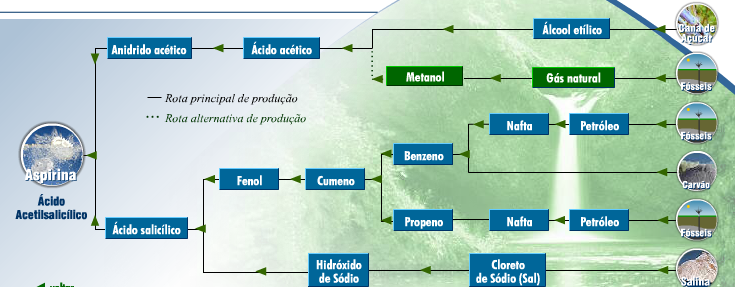
\includegraphics[width=1.10\textwidth]{figuras/abiquim.png}
\end{center}
\caption{Cadeia industrial da produção de Aspirina\R. (Fonte: ABIQUIM, 2009.~\cite{abiquim})}
\label{fig:abiquim}
\end{figure}

\subsection{Mecanismo de ação da Aspirina}

O ácido acetilsalicílico é um anti-inflamatório não esteroide (AINEs) ou não hormonal (AINHs), tendo
como propriedades analgésica, antipirética e anti-inflamatória. Além disso, possui um efeito
inibitório sobre as plaquetas no sangue e apresenta uma redução de 40\% no infarto do miocárdio
fatal e não fatal.~\cite{Palomo2008}

É usado para o alívio da dor e de quadros febris, tais como resfriados e gripes, para controle da
temperatura e alívio das dores musculares e das articulações. Também é usado nos distúrbios
inflamatórios agudos e crônicos, tais como artrite reumatoide, osteoartrite e espondilite
anquilosante.~\cite{bulaaspirina}

A atuação do ácido acetilsalicílico no organismo é de coibir a ação da ciclo-oxigenase. Essa ação
utiliza as enzimas COX-1 e COX-2, as quais transformam o ácido araquidônico em prostaglandinas, que
são responsáveis por induzir a dor e a febre. Esse ácido araquidônico é oriundo da ação enzimática
da Fosfolipase A2 sobre os fosfolipídios presentes nas membranas celulares. 

A plaqueta, importantíssima no processo de coagulação, é rica em COX-1 que, quando necessário,
produz prostaglandinas que são convertidas em Tramboxane A2 levando à formação de um coágulo. O
processo de coagulação se finda quando a Aspirina\R age na inflamação. Com o cessar da ação da
Aspirina\R no organismo, o processo de coagulação é retomado. Porém, uma vez que as plaquetas não
possuem núcleos elas não podem sintetizar uma nova COX para substituir a que foi inativa pela
Aspirina\R. Daí a ação anti-agregante plaquetária, que é um efeito irreversível. Entretanto, essa
ação irreversível não ocorre no endotélio vascular, pois este tem a capacidade de sintetizar as
novas moléculas. 

Devido a esse efeito inibitório da agregação plaquetária, o ácido acetilsalicílico pode aumentar a
tendência de sangramentos durante e após intervenções cirúrgicas (inclusive cirurgias de pequeno
porte, como por exemplo, extrações dentárias).~\cite{bulaaspirina}

Ademais, ao inibir a COX-2 ocorrerá o efeito anti-inflamatório, que diminuirá a inflamação vascular
no sítio da placa ateromatosa e esta, por sua vez, reduz a infiltração de células mononucleares na
placa de ateroma.~\cite{Grassi2012}

Algumas das funções das prostaglandinas estão na produção do muco estomacal, na coagulação sanguínea
e na manutenção da taxa de filtração glomerular nos rins. Como o fármaco (ácido acetilsalicílico)
inibe as enzimas COXs não há a produção das prostaglandinas, tendo como consequências alguns efeitos
no organismo.  Tais como, a úlcera péptica e uma posterior hemorragia digestiva, dependendo da
gravidade do quadro; a insuficiência renal aguda e problemas na coagulação. 

Após a medicação por via oral, o ácido acetilsalicílico é absorvido de forma rápida e completa no
trato gastrintestinal. Depois de absorvido e durante a sua absorção, o ácido acetilsalicílico é
convertido em ácido salicílico, que é o seu principal metabólito ativo. A quantidade máxima de
fármaco na corrente sanguínea do ácido acetilsalicílico é atingida após 10 a 20 minutos e a do ácido
salicílico após 0,3 a 2 horas. 

O ácido acetilsalicílico e o ácido salicílico possuem uma grande afinidade com as proteínas
plasmáticas, logo eles ligam-se extensivamente com tais proteínas e são distribuídos por todo o
organismo rapidamente.  O ácido salicílico passa para o leite materno e atravessa a placenta.

O ácido salicílico é eliminado principalmente por metabolismo hepático. Seus metabólitos incluem o
ácido salicilúrico, o glicuronídeo salicílico fenólico, o glicuronídeo salicilacílico, o ácido
gentísico e o ácido gentisúrico.

O metabolismo é restringido pela capacidade das enzimas hepáticas, sendo assim a cinética da
eliminação do ácido salicílico é dose-dependente. “A meia-vida de eliminação varia de 2 a 3 horas
após doses baixas até cerca de 15 horas com doses altas”~\cite{bulaaspirina}. O ácido salicílico e
seus metabólicos são excretados predominantemente por via renal. 

É importante frisar que esses anti-inflamatórios não esteroides (AINEs), do qual o ácido
acetilsalicílico faz parte, apenas inibem a produção de prostaglandinas na inflamação, mas eles não
cessam a mesma.

\subsection{Medicamentos de referência, genéricos e similares}\label{refgensim}

No mercado farmacêutico, medicamentos com o mesmo princípio ativo podem surgir com diferentes marcas
ou classificações. No caso do ácido acetilsalicílico, algumas são associadas a outras substâncias
como cafeína ou vitamina C. Outras possuem revestimentos de cápsula que buscam diminuir a agressão ao
sistema digestivo.~\cite{prade2006}

Com essas diferenças, os remédios são classificados como referência, genérico e similar. Os
medicamentos de referência, que também são conhecidos como “de marca”, são remédios que possuem
eficiência terapêutica, com qualidade e seguranças comprovadas cientificamente. São registrados
juntamente à Agência Nacional de substância Sanitária. Geralmente são medicamentos com novos
princípios ativos o que trazem novidades para o tratamento da doença.

Já os similares, além de possuir o mesmo princípio ativo do medicamento de referência, possui uma
identificação de nome comercial ou marca. A diferença é apresentada em alguns aspectos como
embalagem, rótulo, tamanho, validade e forma do produto. De acordo com a regulamentação da ANVISA,
dado uma prescrição médica os medicamentos de referência não podem ser substituídos por similares.

Para a possibilidade de troca desses medicamentos, ou seja, serem intercambiáveis, eles devem
apresentar um dos três testes: bioequivalência, biodisponibilidade e bioisenção. O estudo de
bioequivalência é sempre realizado entre o medicamento de referência e o estudado. Estas análises
tem o intuito de reafirmar a igualdade entre os produtos, proporcionando segurança e
eficiência.~\cite{ache2015}

\subsection{Titulação}\label{titulacao}

``Titulação é um procedimento no qual a quantidade de analito de uma amostra é determinada
adicionando-se uma quantidade conhecida de um reagente que reage completamente com o analito de uma
forma bem definida'' (HAGE, CARR. 2012)~\cite{Hage2012}.

Titulações volumétricas compreendem a medida de volume de uma solução padrão (de concentração
conhecida) necessária para reagir completamente com o analito.~\cite{Skoog2014}

Em uma titulação ácido-base, o titulado (analito) é um ácido e o titulante (solução ou composto com
os metros conhecidos) é uma base, ou vice-versa. Para saber quando e quanto de todo o analito
reagiu, é necessário adicionar um indicador ácido-base, uma substância química que muda de cor em
uma faixa conhecida de pH, ajudando a detectar o ponto estequiométrico ou ponto de equivalência.

``O ponto de equivalência é o ponto teórico alcançado quando a quantidade adicionada do titulante é
quimicamente equivalente à quantidade de analito na amostra''~\cite{Skoog2014}. O ponto final é o
ponto onde ocorre visualmente a percepção de alterações físicas (cor ou turbidez) pelo observador.

“Entre o ponto final da titulação e o ponto estequiométrico (teórico) sempre existirá uma pequena
diferença de volume do titulante chamada de Erro de Titulação”.~\cite{Ruy1999}

A reação de neutralização do AAS é dada abaixo:

\begin{center}
    \ce{C8O2H7COOH + NaOH -> C8O2H7COONa + H2O}
\end{center} 

Segundo Skoog et al. (2014), na titulação de um ácido fraco (HA) com uma base forte (\ce{NaOh} ou
\ce{KOH}) ocorrem as seguintes etapas:

\begin{enumerate}
    \item No início, a solução contém somente o analito, ácido fraco.
    \item Com a adição do titulante (até antes do ponto de equivalência), a solução contém uma série
        de tampões, entre a base conjugada formada da reação e o ácido fraco residual que permanece.
    \item No ponto de equivalência, a solução contém apenas o conjugado do ácido (um sal).
    \item Após o ponto de equivalência, o excesso de titulante básico reprime o caráter ácido ou
        alcalino do sal formado, produto da reação, sendo o pH resultante da concentração do excesso
        de titulante.
\end{enumerate}

\begin{figure}[H]
\begin{center}
    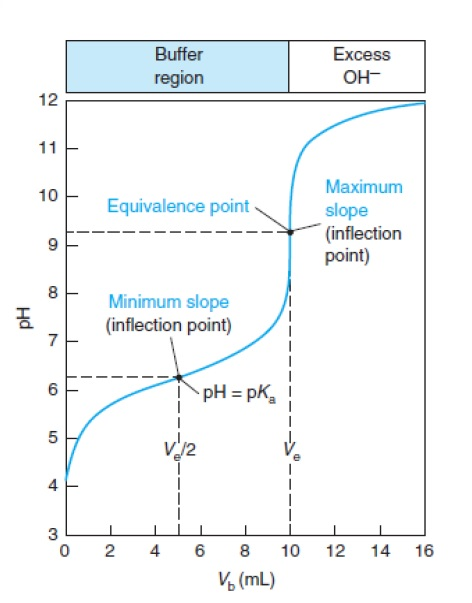
\includegraphics[scale=.9]{figuras/titulacao.jpg}
\end{center}
\caption{Curva de titulação Ácido fraco $\times$ Base forte}
\label{fig:curva_titulacao}
\end{figure}

     \chapter{Materiais e Métodos}\label{sec:mat}
     \section{Materiais}\label{sub:Materiais}
     
     \begin{tabular}{l l}
         \toprule
         \multicolumn{1}{c}{\textbf{Materiais}} & \multicolumn{1}{c}{\textbf{Reagentes}} \\
         \midrule
     \tabitem Almofariz com pistilo & \; \tabitem Água destilada \\
     \tabitem Balão volumétrico 1 L & \multirow{2}{*}{%
         \begin{tabular}{l}
     \tabitem Comprimidos:  \\
     Aspirina$^{\tiny{\textregistered}}$, 
     Melhoral\R, Genérico e AAS Infantil \end{tabular}}\\

     \tabitem Balança analítica & \\
     \tabitem Bastão de vidro & \; \tabitem Etanol comercial \\
     \tabitem Bureta & \; \tabitem Indicador fenolftaleína 0,1\% \\
     \tabitem Béqueres & \; \tabitem Solução padrão de \ce{NaOH} 0,100 mol/L \\
     \tabitem Conta gotas & \\
     \tabitem Erlenmeyer & \\
     \tabitem Espátulas  & \\
     \tabitem Pipeta volumétrica 10 mL  & \\
     \tabitem Pisseta  & \\
     \tabitem Provetas: 50, 100 e 500 mL  & \\
     \tabitem Suporte universal com garra e mufa  & \\
     \bottomrule
     \end{tabular}\hfill\

     \section{Métodos}\label{sub:metodos}

     \subsection{Experimento 1}\label{exp1}

     \subsubsection{Procedimento A}\label{ProcedimentoA}

     Diluiu-se uma solução de \ce{NaOH} 0,2 M afim de obter-se uma solução 0,1 M. Em uma proveta de 500 mL 
     ambientada, mediu-se 500 mL da solução 0,2 M, pipetando-se no final para maior precisão. 
     Transferiu-se quantitativamente o que estava na proveta para um balão volumétrico de 1 L, ou seja, 
     lavou-se as paredes da proveta três vezes com água destilada até garantir que toda a solução havia sido 
     transportada. Completou-se o volume do balão volumétrico até o menisco e homogeneizou-se a 
     solução, invertendo o recipiente tampado, verticalmente, várias vezes. Esta solução será o titulante.

     Foi preparada, com o uso de provetas, 300 mL de um solução 1:1 de etanol comercial e água destilada, 
     que seria o solvente utilizado para dissolver os comprimidos. 

     \subsubsection{Procedimento B}\label{ProcedimentoB}

     Um comprimido de cada medicamento foi pesado em balança analítica e os valores foram anotados. Os 
     comprimidos foram macerados em almofariz com o uso de pistilo e da massa de cada um foi pesada,
     em placa de Petri, uma amostra de 0,100g. Essa amostra foi dissolvida em 50 mL de solvente, em um béquer
     com agitação até a solubilização e posteriormente dividida em quatro amostras de 10 mL, que foram 
     transferidas para erlenmeyers utilizando-se pipeta volumétrica. Foram adicionadas duas gotas de 
     fenolftaleína a cada uma das quatro amostras, as quais serão os titulados.

     \subsubsection{Procedimento C}\label{ProcedimentoC}

     Transferiu-se o titulante para a bureta de 50 mL até zerá-la e deu-se início à titulação de ácido 
     acetilsalicílico com a solução de \ce{NaOH}. O processo de gotejamento do titulante permaneceu até 
     o aparecimento de uma coloração rósea no titulado que persistisse. Anotou-se o volume de titulante gasto 
     para cálculos posteriores. Esse processo foi repetido nas quatro amostras de cada um dos comprimidos.

     \subsection{Experimento 2}\label{exp2}

     Devido a inconsistências encontradas nos cálculos do experimento 1 (\ref{exp1}), foi decidido realizar 
     mais um experimento com algumas ligeiras mudanças nos procedimentos.
     
     \subsubsection{Procedimento A}\label{ProcedimentoA2}

     Para preparação do titulante (solução de \ce{NaOH} 0,1 M), prosseguiu-se da mesma forma que no procedimento
     \ref{ProcedimentoA}. Já o solvente, foi preparado de maneira similar, porém, em maior quantidade.

     \subsubsection{Procedimento B}\label{ProcedimentoB2}

     Como em \ref{ProcedimentoB}, um comprimido de cada medicamento foi pesado e macerado. Os comprimidos 
     macerados foram divididos em três amostras de 0,1000g e cada amostra foi dissolvida em 40 mL de 
     solvente, que foi transferido para um erlenmeyer, utilizando proveta, com agitação até solubilização. 
     Foram necessários dois comprimidos de AAS Infantil para obtenção das três amostras.
     Foram adicionadas três gotas de fenolftaleína a cada uma das três amostras, as quais serão os titulados.

     \subsubsection{Procedimento C}\label{ProcedimentoC2}

     Foi feita a titulação do ácido acetilsalicílico com a solução de \ce{NaOH} como especificado 
     em \ref{ProcedimentoC}. Esse processo foi repetido nas três amostras de cada um dos comprimidos.

 \chapter{Custos}\label{sec:Custos}
 \begin{table}[H]\label{t:custos}
     \centering
     \begin{tabular}{|c | c| }
         \hline
         \textbf{Material} & \textbf{Valor (R\$)} \\
         \hline
         Almofariz com pistilo & 35,00\\ \hline
         Balança analítica & 4700,00 \\ \hline
         Comprimidos de AAs 
         \par(referência, genérico e similar) & 20,00 \\ \hline
         Erlenmeyer 125mL & 9,00 \\ \hline
         Etanol comercial & 80,00 \\ \hline
         Hidróxido de Sódio (\ce{NaOH}) & 20,00 \\ \hline
         Indicador Fenolftaleína 0,1\% & 30,00 \\ \hline
         Proveta 50mL & 8,00 \\ \hline
         \textbf{TOTAL} & \textbf{4902,00} \\ \hline
     \end{tabular}
     \caption{Custos}
 \end{table}

\chapter{Resultados}\label{resultadosk}

Equações utilizadas

\begin{equation}\label{ncv}
     n = \frac{C}{V} 
\end{equation}
onde
\begin{itemize}
    \item[$n$ :] número de mols
    \item[$C$ :] Concentração molar, mol/L
    \item[$V$ :] Volume, L
\end{itemize}

\begin{equation}\label{massamolar}
    MM = \frac{m}{n} 
\end{equation}
onde
\begin{itemize}
    \item[$MM$ :] Massa molar, g/mol
    \item[$m$ :] massa, g
    \item[$n$ :] número de mols
\end{itemize}


\bigskip
Dados gerais

\begin{itemize}
     \item Massa molar de ácido acetilsalicílico: 180,157 g/mol
     \item Concentração da solução \ce{NaOH}(titulante): 0,1 mol/L
     \item Volume de titulante (bureta): 50 mL
     \item Quantidade de NaOH (bureta): 2 mol, obtido da equação \eqref{ncv}
\end{itemize}

\section{Experimento 1}\label{res_exp1}

% Tabela pesagem
\begin{table}[H]\label{t:peso_1}
    \centering
    \begin{tabular}{l c c}
       \toprule
       Medicamento & $m_{comprimido}$ (g) & $m_{amostra}$ (g) \\
       \midrule
       Aspirina\R & 0,600 & 0,099  \\
       Genérico & 0,610 & 0,100  \\
       Melhoral & 0,587 & 0,101 \\
       AAS Infantil & 0,164 & 0,100 \\
        \bottomrule
    \end{tabular}
    \caption{Informações das pesagens no primeiro experimento}
\end{table}

% Tabela de dados titulados
\begin{table}[H]\label{titulacao_exp1}
    \centering
    \begin{tabular}{l c c c c c}

        \toprule
        Medicamento & $v_1$  & $v_2$ & $v_3$ & $v_4$ & $v_{\textrm{méd}}$ \\
        \midrule
        Aspirina\R     & 1,0 & 1,1 & 1,2 & 1,1 & 1,100 \\
        Genérico     & 1,0 & 1,0 & 1,0 & 0,9 & 0,975  \\
        Melhoral     & 1,0 & 1,0 & 1,0 & 1,1 & 1,025\\
        AAS Infantil & 0,7 & 1,0 & 0,8 & 0,7 & 0,800\\
       \bottomrule

    \end{tabular}
    \caption{Volumes obtidos na titulação, em mL}
\end{table}

\begin{table}[H]\label{res_calculados_exp1}
    \centering
    \begin{tabular}{l r c c c }
        \toprule
        Medicamento & $n_{\textrm{AAS}}$ &$m_{AAS}$(titulado)& 
        $m_{\textrm{AAS}}$(exp) & $m_{\textrm{AAS}}$ (bula) \\

        \midrule
        Aspirina\R     & $1,1\cdot 10^{-4}$   &19,817 & 600,52 & 500\\
        Genérico     & $9,75\cdot 10^{-5}$  & 17,565 & 535,74 & 500 \\
        Melhoral     & $1,025\cdot 10^{-4}$ & 18,466 & 536,61 & 500 \\
        AAS Infantil & $8,0\cdot 10^{-5}$   & 14,413 & 118,18 & 100 \\
        \bottomrule
    \end{tabular}
    \caption{Resultados calculados}
\end{table}

onde
\begin{itemize}
    \item[] $n_{AAS}$: número de mol de AAS em uma alíquota  de 10 mL da amostra. Obtido
        com a equação \eqref{ncv}
    \item[] $m_{AAS}$ (titulado): massa de AAS em uma alíquota de 10 mL da amostra, em mg.
        Obtida da equação \eqref{massamolar}
    \item[]$m_{AAS}$ (exp): massa calculada de AAS na massa total do comprimido, em mg
    \item[] $m_{AAS}$ (bula): massa de AAS no comprimido informada pela bula, em mg
\end{itemize}


\begin{table}[H]\label{porcentagem1}
    \centering
    \begin{tabular}{l c c}
        \toprule
        Medicamento & Experimental & Bula \\
        \midrule
        Aspirina\R     & 100,087 & 83,333 \\
        Genérico     & 87,826  & 81,967 \\
        Melhoral     & 91,416  & 85,179 \\
        AAS Infantil & 72,061  & 60,976 \\
        \bottomrule
    \end{tabular}
    \caption{Massa de AAS por massa do comprimido, em porcentagem}
\end{table}

\section{Experimento 2}\label{res_exp2}

\begin{table}[H]\label{t:peso_2}
    \centering
    \begin{tabular}{l c c c c}
       \toprule
       Medicamento & $m_{comprimido}$ (g) &$m_{amostra \, 1}$ (g) &
       $m_{amostra \, 2}$ (g) & $m_{amostra\, 3}$ (g)\\
       \midrule
       Aspirina\R     & 0,6029 & 0,0996 & 0,0998 & 0,0997  \\
       Genérico     & 0,6068 & 0,0996 & 0,0999 & 0,1003  \\
       Melhoral     & 0,6191 & 0,1000 & 0,0995 & 0,0998 \\
       AAS Infantil & 0,1622 & 0,0999 & 0,1000 & 0,1000 \\
        \bottomrule
    \end{tabular}
    \caption{Informações das pesagens no segundo experimento}
\end{table}

\begin{table}[H]\label{titulacao_exp2}
    \centering
    \begin{tabular}{l c c c c}

        \toprule
        Medicamento & $v_1$  & $v_2$ & $v_3$ &  $v_{\textrm{méd}}$ \\
        \midrule
        Aspirina\R   & 4,4 & 4,3 & 4,4 & 4,367 \\
        Genérico     & 4,2 & 4,3 & 4,3 & 4,267 \\
        Melhoral     & 4,2 & 4,3 & 4,3 & 4,267 \\
        AAS Infantil & 3,3 & 3,3 & 3,3 & 3,300 \\
       \bottomrule

    \end{tabular}
    \caption{Volumes obtidos na titulação, em mL}
\end{table}

\begin{table}[H]
    \centering
    \begin{tabular}{c c c c}
        \toprule
        Amostra & $n_{AAS}$ & $m_{AAS}$ (titulado) & $m_{AAS}$ (exp) \\
        \midrule
        A1 & $4,4\cdot 10^{-4}$ & 79,269 & 479,833 \\
        A2 & $4,3\cdot 10^{-4}$ & 77,468 & 467,988\\
        A3 & $4,4\cdot 10^{-4}$ & 79,269 & 478,635 \\
        \bottomrule
    \end{tabular}
    \caption{Resultado da titulação da Aspirina\R}
    \label{res_aspirina}
\end{table}

\begin{itemize}
    \item $m_{AAS,\; med}$ (exp) $= 475,485$ mg
\end{itemize}

\begin{table}[H]
    \centering
    \begin{tabular}{c c c c}
        \toprule
        Amostra & $n_{AAS}$ & $m_{AAS}$ (titulado) & $m_{AAS}$ (exp) \\
        \midrule
        G1 & $4,2\cdot 10^{-4}$ & 75,666 & 460,985 \\
        G2 & $4,3\cdot 10^{-4}$ & 77,468 & 470,543 \\
        G3 & $4,3\cdot 10^{-4}$ & 77,468 & 468,667 \\
        \bottomrule
    \end{tabular}
    \caption{Resultado da titulação do genérico}
    \label{res_generico}
\end{table}

\begin{itemize}
    \item $m_{AAS,\; med}$ (exp) $= 466,732$ mg
\end{itemize}

\begin{table}[H]
    \centering
    \begin{tabular}{c c c c}
        \toprule
        Amostra & $n_{AAS}$ & $m_{AAS}$ (titulado) & $m_{AAS}$ (exp) \\
        \midrule
        M1 & $4,2\cdot 10^{-4}$ & 75,666 & 468,448 \\
        M2 & $4,3\cdot 10^{-4}$ & 77,468 & 482,011 \\
        M3 & $4,3\cdot 10^{-4}$ & 77,468 & 480,562 \\
        \bottomrule
    \end{tabular}
    \caption{Resultado da titulação do Melhoral}
    \label{res_melhoral}
\end{table}

\begin{itemize}
    \item $m_{AAS,\; med}$ (exp) $= 477,007$ mg
\end{itemize}

\begin{table}[H]
    \centering
    \begin{tabular}{c c c c}
        \toprule
        Amostra & $n_{AAS}$ & $m_{AAS}$ (titulado) & $m_{AAS}$ (exp) \\
        \midrule
        I1 & $3,3\cdot 10^{-4}$ & 59,452 & 96,527 \\
        I2 & $3,3\cdot 10^{-4}$ & 59,452 & 96,431 \\
        I3 & $3,3\cdot 10^{-4}$ & 59,452 & 96,431 \\
        \bottomrule
    \end{tabular}
    \caption{Resultado da titulação do AAS Infantil}
    \label{res_infantil}
\end{table}

\begin{itemize}
    \item $m_{AAS,\; med}$ (exp) $= 96,463$ mg
\end{itemize}

Das tabelas \ref{res_aspirina} a \ref{res_infantil}

\begin{itemize}
    \item[] $n_{AAS}$: número de mol de AAS em uma amostra dissolvida em 40 mL de solvente. Obtido
        com a equação \eqref{ncv}
    \item[] $m_{AAS}$ (titulado): massa de AAS em uma amostra dissolvida 
        em 40 mL de solvente, em mg. Obtida da equação \eqref{massamolar}
    \item[]$m_{AAS}$ (exp): massa calculada de AAS na massa total do comprimido, em mg
\end{itemize}

\begin{table}[H]\label{porcentagem2}
    \centering
    \begin{tabular}{l c c}
        \toprule
        Medicamento & Experimental & Bula \\
        \midrule
        Aspirina\R   & 78,866 & 82,932 \\
        Genérico     & 76,917  & 82,399 \\
        Melhoral     & 77,049  & 80,762 \\
        AAS Infantil & 59,472  & 61,652 \\
        \bottomrule
    \end{tabular}
    \caption{Massa de AAS por massa do comprimido, em porcentagem}
\end{table}

\chapter{Cronograma}\label{sec:Cronograma}

\begin{table}[ht]
\label{cronograma}
\caption{Cronograma planejado}
\centering

\begin{tabular}{|P{6cm}|c|c|c|c|c|c|}
    \hline
    \multirow{2}*{\textbf{Atividades}} & \multicolumn{6}{c|}{\textbf{Semanas}} \\ \cline{2-7}
    & 1 & 2 & 3 & 4 & 5 & 6 \\
    \hline
    Revisão de literatura                & \textbf{X} & \textbf{X} & \textbf{X} &   &   &   \\
    \hline
    Preparação e separação dos materiais & \textbf{X} & \textbf{X} &   &   &   &   \\
    \hline
    Montagem do experimento              & \textbf{X} & \textbf{X} & \textbf{X} &   &   &   \\
    \hline
    Coleta de dados                      &   &   & \textbf{X} & \textbf{X} & \textbf{X} &   \\
    \hline
    Apresentação do projeto              &   &   &   &   &   & \textbf{X} \\
    \hline
    
\end{tabular}

\end{table}



%==============================================================================
% Incluindo bibliografia
%\bibliographystyle{plain}             % estilo para labels em numeros
%\bibliographystyle{alpha}             % estilo para labels em iniciais
\bibliographystyle{abntex2-num}           % estilo para referências usando ABNT, 

%inclui Referências Bibliográficas
\referencias
\bibliography{bibliografia/b}

%==============================================================================
% Fim do texto
\end{document}
